\documentclass[10pt]{article}
\usepackage{graphicx}
\usepackage[T1]{fontenc}
\usepackage{txfonts}
\setcounter{secnumdepth}{0}
\usepackage[affil-it]{authblk}   % author affiliation
\usepackage{lineno} %line numbers
\usepackage[a4paper, total={6.5in, 8.5in}]{geometry} % set page size
\usepackage{setspace}
\usepackage{multicol}

\usepackage[authormarkup=none]{changes}
%\usepackage[final]{changes}
\definechangesauthor[name={Jess}, color=blue]{J}
\definechangesauthor[name={Iva}, color=purple]{I}
\definechangesauthor[name={Aaron}, color=green]{A}

\begin{document}

\title{Demographic Bias in Human Cell Studies }
\author{Jessica Snyder\textsuperscript{1}, Iva Bojic\textsuperscript{1,2}, Aaron Gerow\textsuperscript{3}, Carlo Ratti  \textsuperscript{1,2 } \\ \textsuperscript{1}Massachusetts Institute of Technology, SENSEable City Lab \\ \textsuperscript{2}Singapore-MIT Alliance for Research and Technology \\ \textsuperscript{3}University of Chicago, Computation Institute}

\maketitle

\begin{multicols}{2}
Breast cancer treatments are shaped by the research tools used to understand the disease. As these tools become increasingly focused, it is important to understand how inclusive they are of treatment populations. The use of human cell lines, in particular, in the development of cancer treatments poses serious questions about representation. Looking at the demographics of cell lines in published research, we find a discernible bias for the majority patient ethnicity.

From 1999 to 2013, the population of female breast cancer patients has been proportionally shrinking (figure 1A). The population-level decrease indicates that environmental stressors triggering breast cancer are likely being reduced. One explanation is that decreased prescription of a hormone-replacement therapy (HRT), which is shown to increase white and hispanic patient's risk of breast cancer by >20\% \cite{million2003breast}. HRT was not, however, found to increase risk for black women. Because HRTs were limited in 2002, the rate of breast cancer incidence among white, hispanic and Native American women have fallen, while the rate for black and Asian women increased over the same time. Looking simply at etnicity, the breast cancer population is a heterogenous disease, having sub-types with their own risk factors and pathologies. 

The prognosis for women diagnosed with breast cancer has improved, in part due to advances in screening, early detection, and increasing survival rates, especially for women under 50 years old \cite{etzioni2003case}. Of deaths caused by breast cancer, black women had the highest rate from 1999-2013, higher than white women, who are more likely to be diagnosed (figure 1B). This might be due to later stages of diagnosis and more aggressive tumor sub-types, both of which disproportionately affect black patients \cite{batina2013variation}. Characterization of each breast cancer sub-type provides the scientific basis for treatment options, like it already has for the most common forms as shown by the increasing survival rate. Our question is, which ethnicities, as a proxy for tumor sub-types, are represented in the medical research?%, specifically breast cancer cell lines?

% This paragraph reads as if breast cancer cell lines aren't cell lines. first BC cell line in 1958, but first cell line in 1974. // AG
The first breast cancer cell line was donated by a 74 year old female patient in 1958, named BT-20. BT-20 remained the only breast cancer cell line for more than a decade, until other cells were cultured from white female patients in the 1970s. A list of all human cell lines -- not just cancer cells -- was developed in previous work to assess cell line authentication and quality control, inventory cell line features \cite{yu2015resource}. While researchers conceivable have access to the full range of cell lines, in practice, many lines are used as standards to compare new findings to previous work. The first cell line derived from a black patient's biopsy was in 1974, followed by the first Asian breast cancer cell lines 20 years later in 1994 and the first Hispanic line was developed in 1995. There are currently no Native American breast cancer cell lines currently available. To date, 134 breast cancer cell lines derived from humans are available. Of which, 68 have declared an ethnicity for the donor. Of those, the donors include a majority of 50 lines from white donors, 12 from black donors, 4 from Hispanic donors, and 2 from Asian donors. %%% Mix up here 

In published research, citations to cell lines suggest that the desire for standards exerts a homogenizing force. Among 1.2 million publications from 1975 to 2016, cited a human cell line derived from breast cancer (see Appendix; Methods \& Materials). 85.6\% cited a cell line from a white donor. The next most frequent cell line citation was to donors of unknown ethnicity, 8.8\%, then black donors at 5.0\%, and at order of magnitude less publications cited cell lines from Asian donors at 0.5\%, and another order of magnitude less were declared Hispanic cell lines at 0.1\%. There were no citations of lines from Native American patients as none were available (figure 1C).

Publication are the typical output of research communities, but scientific findings are also made in commercial settings. Like publications, U.S. Patents show evidence of developing treatments. From 2001 to 2015 shows, the majority of cell lines in patents were from a white donor, the second most being black. No other ethnicities were represented in patents (figure 1D).

Using statistics from the U.S. CDC, for each ethnic population, the fraction of indidence and death was calculated. Similarly, for each ethnicity, the fraction of cited cell lines in publications and patents was calculated. These proportions were used to estimate bias in research. First, there is a bias in treatment efficacy: subtracting each ethnicity's fraction in the incidence from the death population, black patient are the only group for which the death population is greater than incidence, by 0.4\%.%Am I just stupid, but how is this possible? It sounds like more black women are dying of breast than have it. // AG
There is also bias in the publication record: blacks represent about 10\% more of the death population than citations of black cell lines in publications (figure 1F). Whites are the only ethnic group represented more in publications than in the death population, by more than 15\%. This finding is true also for patents, which favor the majority ethnicity (figure 1G). Comparingf the representation of each ethnic group in 2013 shows a more proportional representation of the majority patient ethnicity and dependence on cell model standards, figure 1H. % This final sentence doesn't make sense to me // AG

The use of cell models may hinder generalization of results. More than 50,000 women will be diagnosed with breast cancer between 2010-2020 in the U.S. alone, at a medical cost estimated at \$48 billion \cite{mariotto2011projections, weir2015past}. The National Institutes of Health (NIH) and the National Cancer Institute (NCI) invested a combined \$4.1 billion in breast cancer research from 2012 through 2014. %with the goal of restoring the nation's breast cancer patient population to good health.
Assessments of disease burden and treatment effectiveness are used to guide funding for medical research and policy toward the most productive outcomes \cite{kim2016cancer}. To this end, as black patients comprise more of the death population than incidence, CDC statistics suggests that breast cancer treatment is less effective for black women than women of all other races. Despite the fact that previous studies showed black breast cancer patients presented elevated risk for aggressive, intrinsic factors of breast cancer \cite{huo2009population, reding2012examination}, instead of assigning more resources into research using cell lines from black donors, the opposite is the case: whites are over-represented in research by more than 15\%.

Today, the only available regulative apparatus is found in the US Food and Drug Administration (FDA) which in 1998, when pharmaceutical efficacy was found to be sensitize to genetic factors, responded by implementing the Demographic Rule. The Rule established guidelines for racial and ethnic representativeness during clinical trails. However, clinical trials are one of the final stages of work that often begins with the use of cell models, animal models, and finally human models. Should such guidelines be extended to the preclinical stage? Recent efforts from the NIH to balance sex in cell and animal studies suggests so \cite{clayton2014nih}. The 1993 NIH Revitalization Act aimed to increase representation of women and minorities in clinical trials, but did not address earlier stages of research. Despite multiple calls for action, the publication record continues to neglect ethnic considerations, the effects of which surely permeate later-stage research. While legislative solutions may be too restrictive for all research, prioritizing inclusiveness and diversity in the use of cell lines could be feasibly integrated into review and editorial processes.

Initiatives such as Cancer Moon Shot's database, which catalogs tumor sub-types from the patient populations, could help reduce dependence on standard models, the use of which passively perpetuates the bias in early-stage research, by highlighting patients without effective treatment options \cite{lowy2016cancer}. We hope similar such collaborative approaches can populate the human cell line bank and medical research community to discover the multitude of pathologies involved in breast cancer, alleviating the community's dependence on standards as we realize the potential of personalized medicine.
 
\end{multicols}

\begin{figure}[h!]
\centering
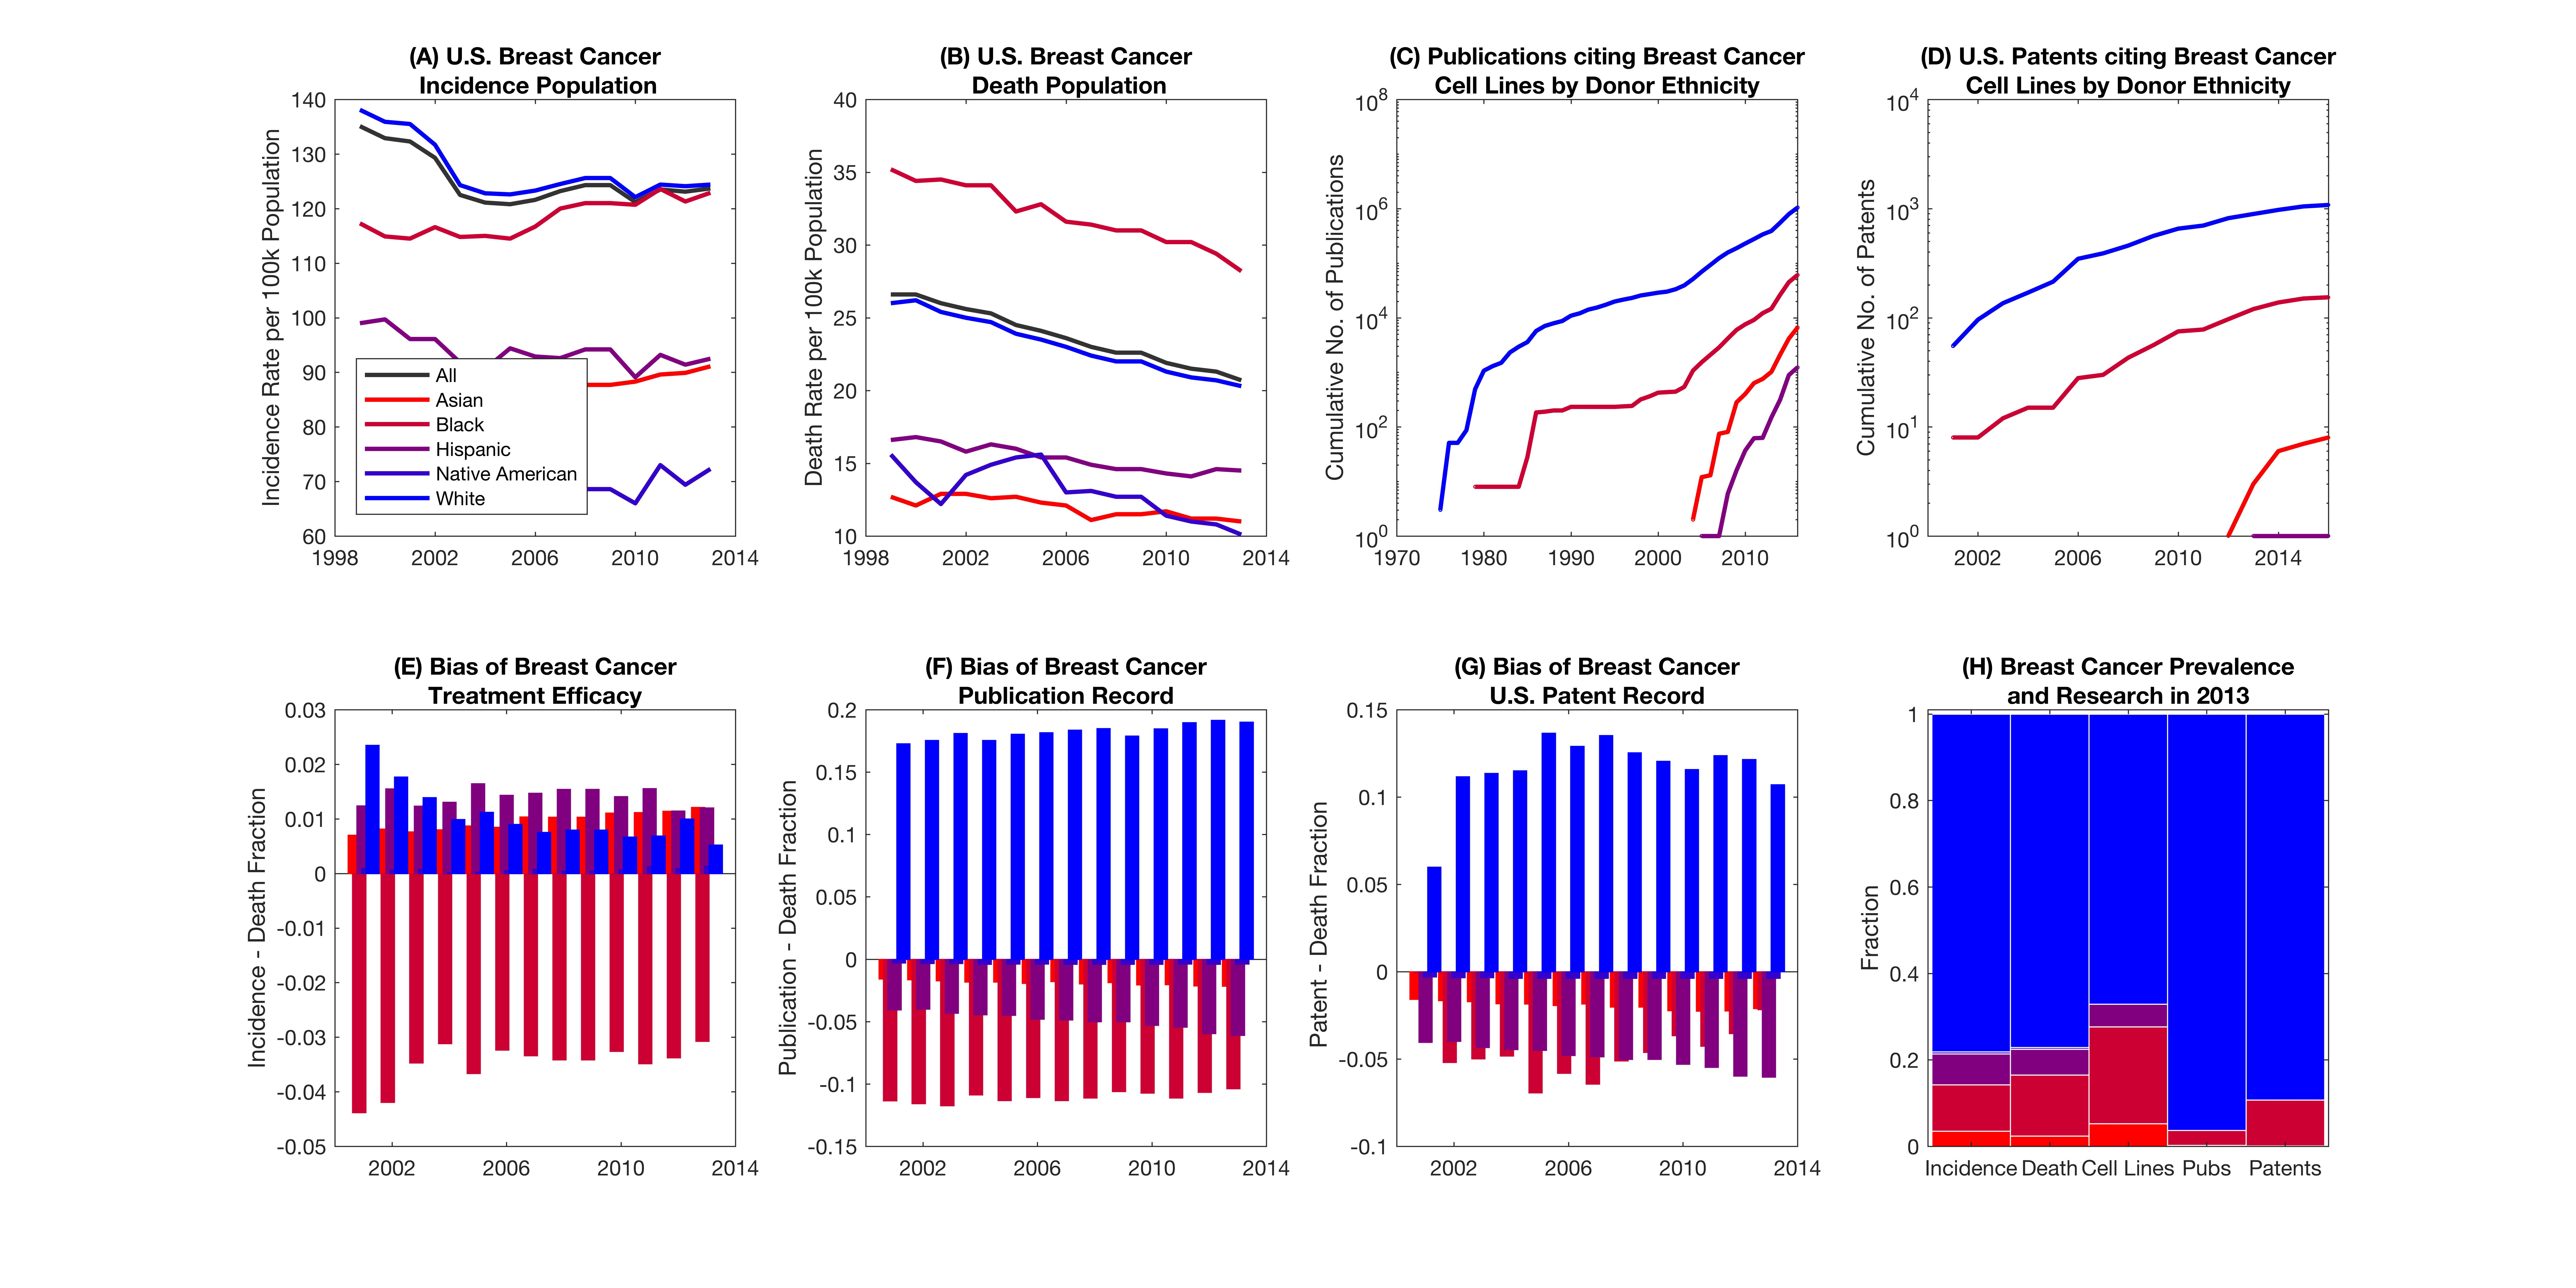
\includegraphics[width=1\columnwidth, trim = {30cm 10cm 30cm 5cm}, clip]{Figures/BreastComposite.jpg}
\caption{\label{PS1} Breast cancer prevalence and research.}
\end{figure}
 
\bibliographystyle{unsrt}
\bibliography{refs}

\section{Appendix}
The same analysis was conducted from prostate and lung cancer. 

\begin{figure}[h!]
\centering
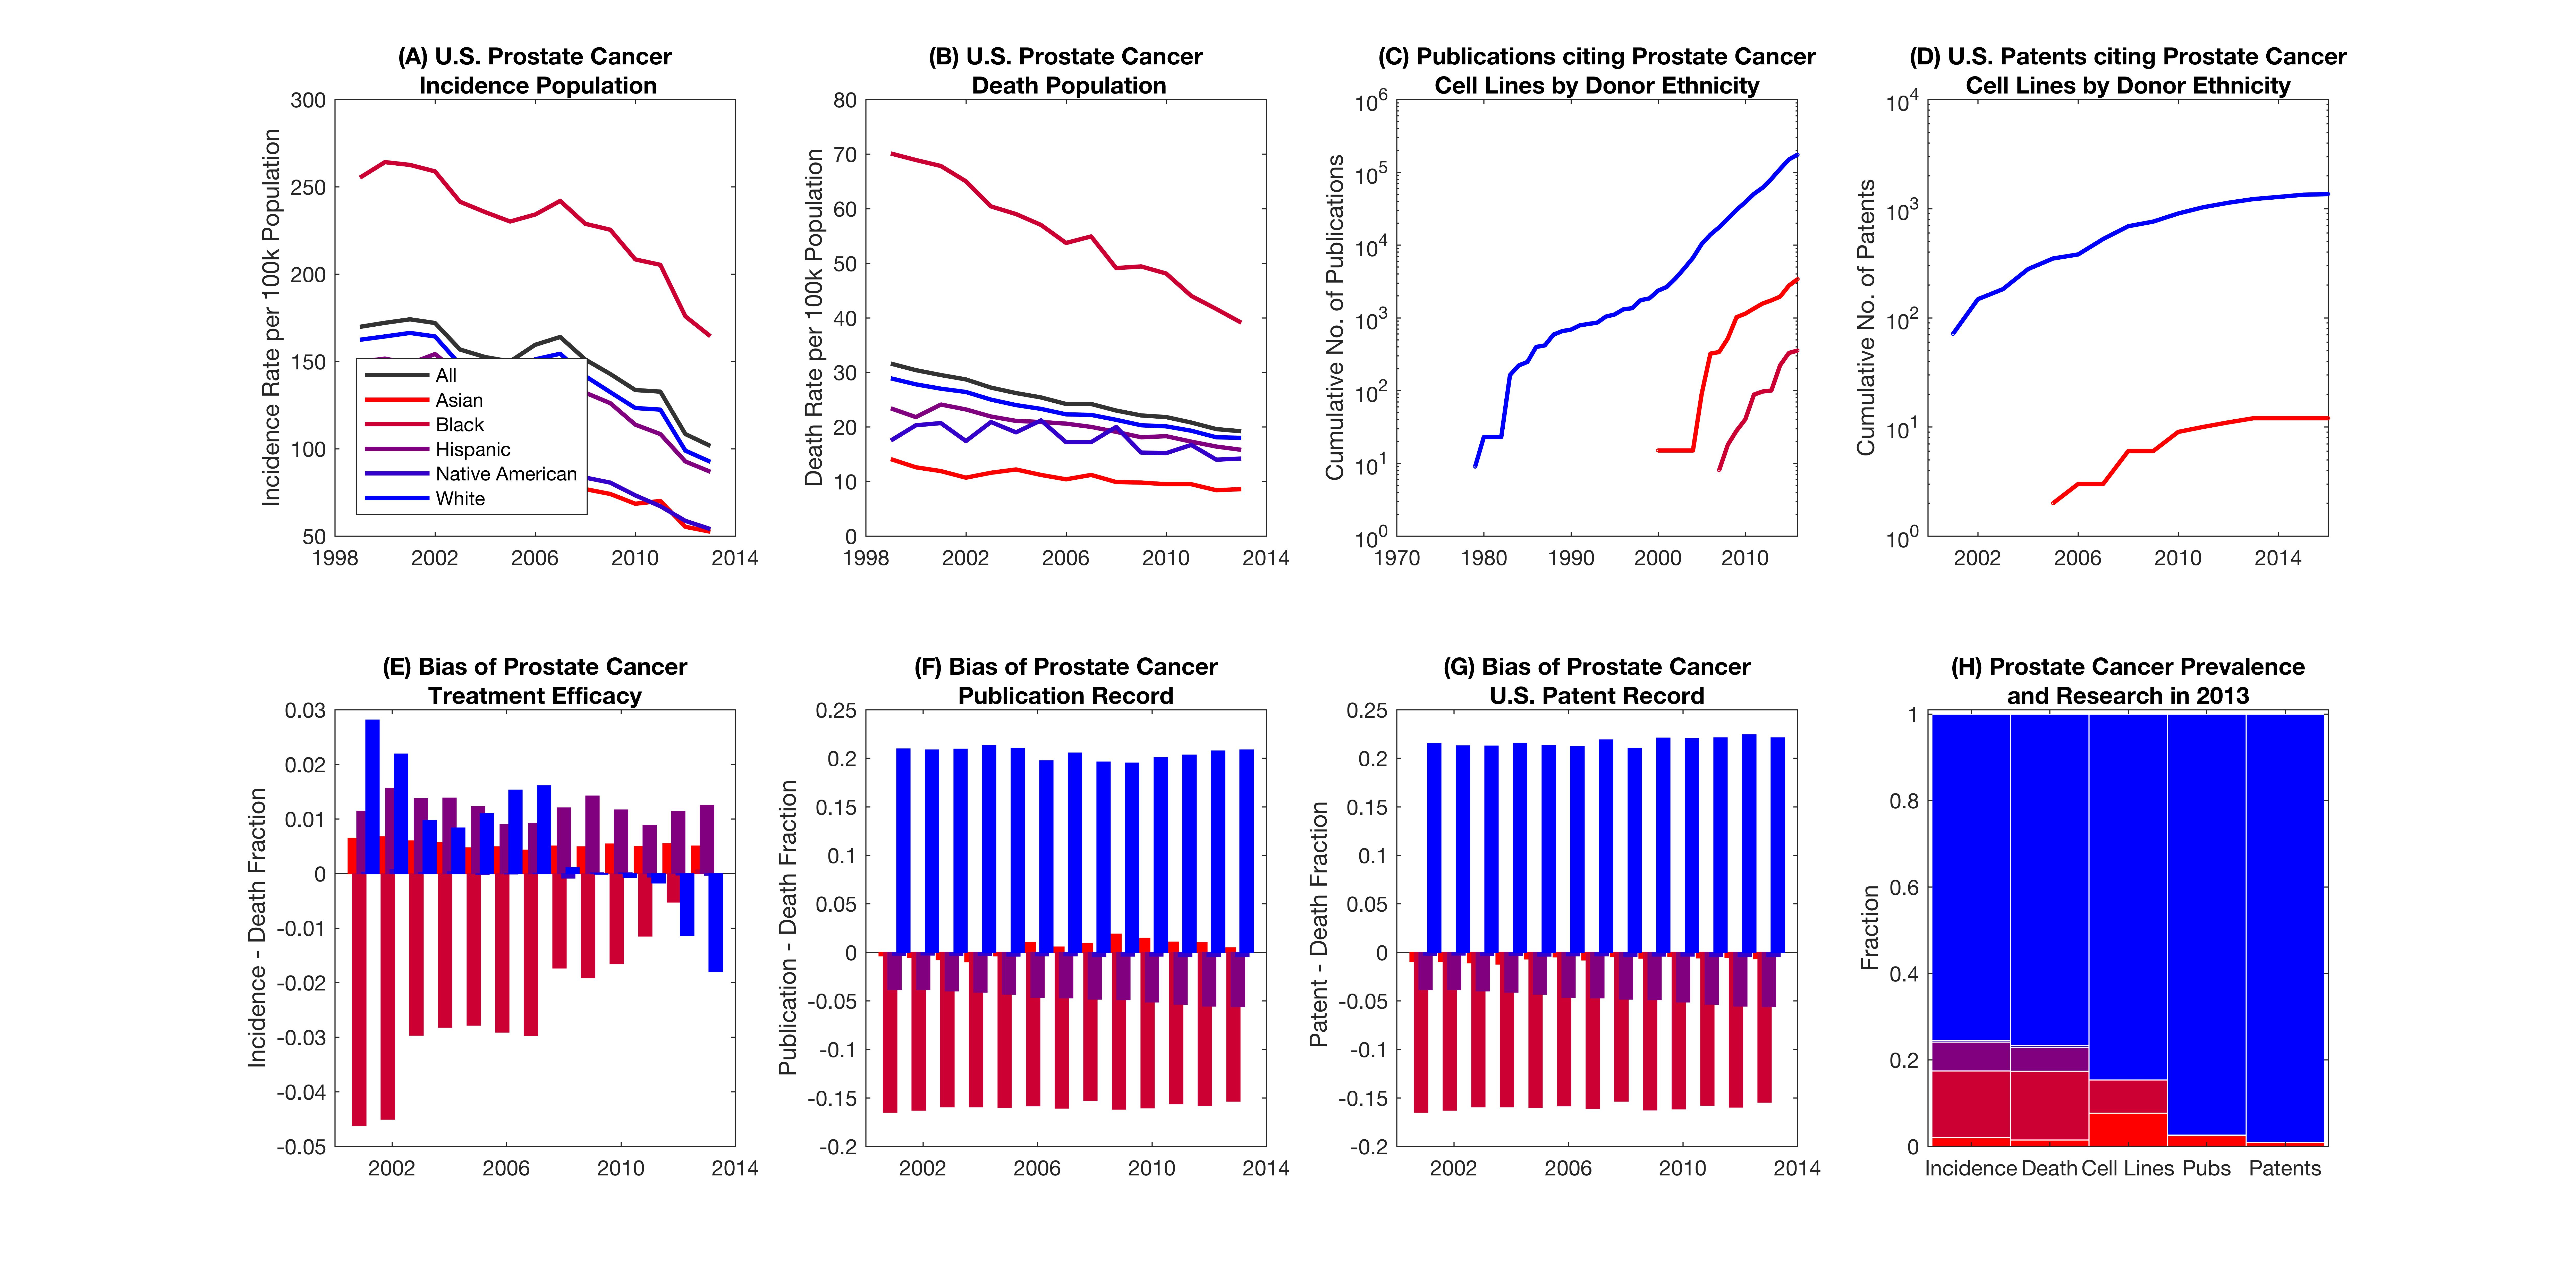
\includegraphics[width=1\columnwidth, trim = {30cm 10cm 30cm 5cm}, clip]{Figures/ProstateComposite.jpg}
\caption{\label{PS2} Prostate cancer}
\end{figure}

\begin{figure}[h!]
\centering
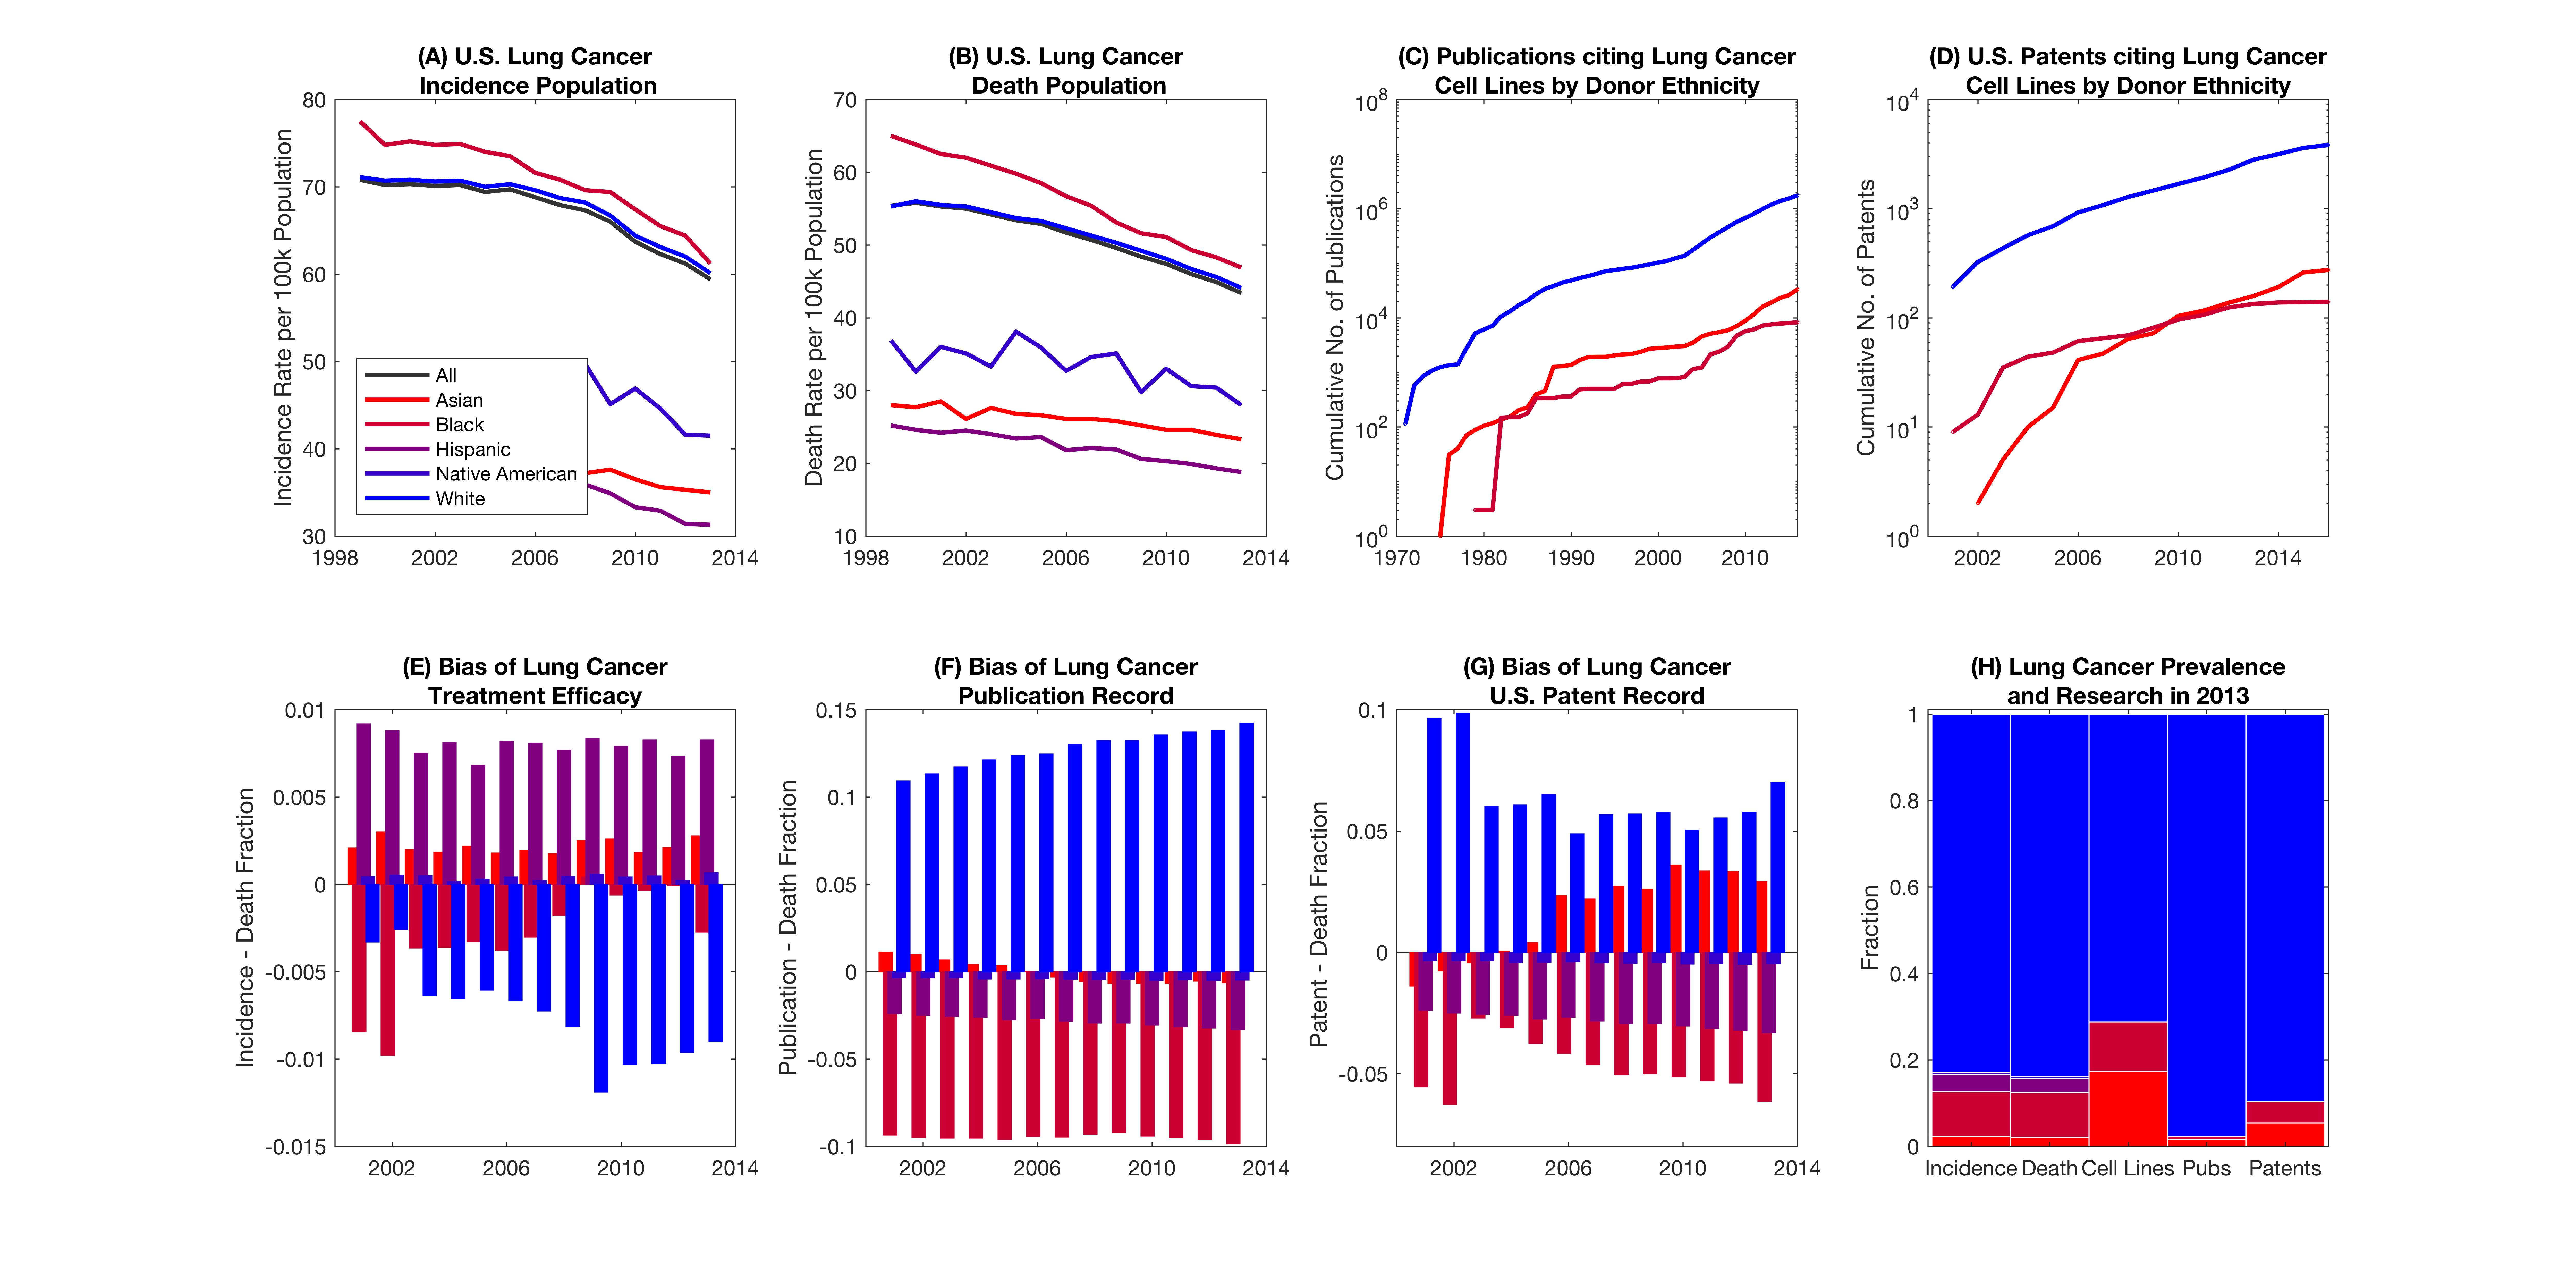
\includegraphics[width=1\columnwidth, trim = {30cm 10cm 30cm 5cm}, clip]{Figures/LungComposite.jpg}
\caption{\label{PS3} Lung cancer.}
\end{figure}

\subsection{Methods \& Materials}
A set of <X> papers publised from 1970 to 2016 were selected from \textsc{medline} by MeSH term and journal. From this set, 169,464 were available for download from PubMed Central and / or SCOPUS. Cell lines included in the supporting data for \cite{yu2015resource} were extracted. 148,177 documents had one or more cell lines, and a total of 2,957,185 citations were found. This included cells observed in different forms (e.g. \textit{MCF 7} vs \textit{MCF/7}). This procedure was also performed on the entirity of the U.S. Patents from 1990 to May, 2015. <X> patents mentioned one or cell lines; there were a total of <X> citations of a cell line. In both data-sets, commonly mis-identified cell names were excluded (eg. \textit{FL} and \textit{TN}). <X> of the excluded lines were breast or prostate cell lines. <X> documents cited at least one cell line, and <X> cited a breast or prostate cancer cell line. The database of cell line citations in publications and patents will be made available online.

\end{document}
